\documentclass[10pt,a4paper]{article}
\usepackage{amsmath}
\usepackage{amssymb}
\usepackage{graphicx}
\usepackage{color}
\usepackage{fancyhdr}
\usepackage{fancyvrb}
\usepackage[margin=3.5cm]{geometry}
\usepackage{framed}
\usepackage{enumerate}
\usepackage{textcomp}
\def\ket#1{\left|#1\right\rangle}
\def\bra#1{\left\langle#1\right|}
\def\braket#1{\left\langle#1\right\rangle}

\definecolor{linkcol}{rgb}{0.0, 0.0, 0.7}
\usepackage[colorlinks=true,urlcolor=linkcol,citecolor=black,linkcolor=linkcol]{hyperref}

\renewcommand{\theequation}{5.\arabic{equation}}
\setcounter{section}{5}
\renewcommand\thesection{\arabic{section}}
\renewcommand\thesubsection{\thesection.\arabic{subsection}}

\fancyhf{}
\lhead{\tiny Y.~D.~Chong (2021)}
\rhead{\scriptsize MH2801: Complex Methods for the Sciences}
\lfoot{}
\rfoot{\thepage}
\pagestyle{fancy}

\begin{document}
\setcounter{page}{31}

\noindent
{\Large \textbf{5. Complex Oscillations}}
\vskip 0.2in

\label{complex-oscillations}

In physics and the other quantitative sciences, complex numbers are
widely used for analyzing oscillations and waves. We begin our study
of this topic with an elementary model called the \textbf{damped
  harmonic oscillator}.

\subsection{The damped harmonic oscillator}
\label{the-damped-harmonic-oscillator}

A particle of mass $m$ moves along one dimension, with $x(t)$ denoting
its displacement at time $t$. It is subject to two forces: a spring
force and a damping force. The spring constant is $k = m\omega_0^2$,
and the damping coefficient is $2m \gamma$.  The parameters $m$,
$\gamma$, and $\omega_0$ are all positive real numbers.

\begin{figure}[ht]
  \centering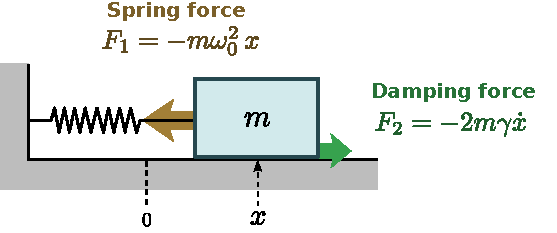
\includegraphics[width=0.6\textwidth]{oscillator}
\end{figure}

According to Newton's second law,
\begin{align}
  m \frac{d^2 x}{dt^2} = F(x,t) = - 2m\gamma \frac{dx}{dt} - m\omega_0^2 x(t).
\end{align}
Dividing by the common factor of $m$, and bringing everything to one
side, gives
\begin{align}
  \frac{d^2 x}{dt^2} + 2\gamma \frac{dx}{dt} + \omega_0^2 x(t) = 0.
\end{align}
This is called the \textbf{damped harmonic oscillator equation}. It is
a second-order ordinary differential equation (ODE), so its general
solution must contain two free parameters. These parameters are
usually (but not necessarily) specified by the initial displacement
$x(0)$ and initial velocity $\dot{x}(0)$.

\begin{framed}\noindent
  \textit{Note}---Sometimes, we write the damped harmonic oscillator
  equation as:
  \begin{align}
    \left[\frac{d^2}{dt^2} + 2\gamma \frac{d}{dt} + \omega_0^2 \right]\, x(t) = 0.
  \end{align}
  The quantity in square brackets is a linear differential operator acting on $x(t)$.  The three terms in the operator correspond to the three ingredients of the damped harmonic oscillator model: (i) a second derivative term stemming from Newton's second law, (ii) a first derivative term representing damping, and (iii) a constant term representing the spring force.

  Writing the differential equation this way emphasizes its linearity,
  a property that is important for finding the solutions, as discussed
  below.
\end{framed}

\subsubsection{Simple harmonic oscillator limit}

For $\gamma = 0$ (zero damping), the system reduces to the
\textbf{simple harmonic oscillator}. From previous physics courses, we
know the general solution is
\begin{align}
  x(t) = A \cos(\omega_0 t + \phi),
\end{align}
where $A$ and $\phi$ are free parameters. This is a sinusoidal
oscillation with amplitude $A$, phase $\phi$, and frequency
$\omega_0$.

The parameter $\omega_0$ comes from the spring constant $k =
m\omega_0^2$. (In fact, the spring constant was parameterized this way
so that the solution ends up with this nice form.) We call $\omega_0$
the \textbf{natural frequency}, meaning the frequency of the
oscillator in the absence of damping or other disturbances.

\begin{framed}\noindent
  \textit{Note}---Some authors call $\omega_0$ the ``angular
  frequency'', reserving the term ``frequency'' for the quantity $f_0
  = \omega_0/2\pi$.  But since we will always deal with $\omega_0$
  rather than $f_0$, we will refer to $\omega_0$ as simply
  ``frequency''.
\end{framed}
  
\subsubsection{Damped oscillations}
\label{damped-oscillations}

For $\gamma > 0$, there is now a damping force opposing the motion of
the oscillator. What form will the solutions take?  Before launching
into the mathematics, let's use our physical intuition to make a
guess.

The damping force does work against the particle (since its sign is
always opposite to the particle's velocity). If the damping force is
very weak, the solution should not be too different from the simple
harmonic oscillator solution---the particle should oscillate around
the equilibrium point $x = 0$ with a frequency of around
$\omega_0$. But the damping force will cause it to lose a bit of
energy every oscillatory cycle, resulting in an oscillation whose
amplitude diminishes slowly over time. In the $t \rightarrow \infty$
limit, all the energy is lost, and $x$ (as well as $\dot{x}$) should
go asymptotically to zero.

So we would guess something like this:

\begin{figure}[ht]
  \centering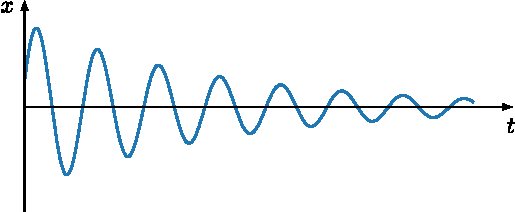
\includegraphics[width=0.65\textwidth]{underdamped_guess}
\end{figure}

\noindent
Let us see if the mathematical analysis agrees with this guess.

\subsection{The complex damped harmonic oscillator equation}
\label{complex-solution}

The variable $x(t)$ is the displacement of the particle, so it ought
to be real. However, a good way to solve the damped harmonic
oscillator equation is to generalize $x(t)$ to complex values.  In
other words, we convert the harmonic oscillator equation into a
complex ODE:
\begin{align}
  \frac{d^2 z}{dt^2} + 2\gamma \frac{dz}{dt} + \omega_0^2 z(t) = 0, \quad z(t) \in \mathbb{C}.
\end{align}
The parameter-counting rule for real ODEs (see Section 1.3)
generalizes to complex ODEs, except that the free parameters should be
complex numbers. In this case, the complex damped harmonic oscillator
equation is a second-order ODE, so its general solution must have two
complex free parameters.

If we can find a solution $z(t)$ for the complex damped harmonic
oscillator equation, then its real part $x(t) = \mathrm{Re}[z(t)]$
would be a solution to the real damped harmonic oscillator equation,
since
\begin{align}
  \frac{d^2 x}{dt^2} + 2\gamma \frac{dx}{dt} + \omega_0^2 x(t) &= \frac{d^2 \mathrm{Re}[z]}{dt^2} + 2\gamma \frac{d \mathrm{Re}[z]}{dt} + \omega_0^2 \, \mathrm{Re}[z(t)] \\
  &= \mathrm{Re}\left[\frac{d^2 z}{dt^2} + 2\gamma \frac{dz}{dt} + \omega_0^2 z(t)\right] \\
  &= 0.
\end{align}
Here, we have used the fact that the $\mathrm{Re}[\cdots]$ operation
can be freely shuffled in or out of derivatives and sums with real
coefficients (see Section 3.1).

\subsubsection{Complex ansatz}
\label{complex-ansatz}

We now aim to derive the general solution for the complex damped
harmonic oscillator equation.

First, note that the equation is linear. This means that for any two
solutions $z_1(t)$ and $z_2(t)$, a linear superposition
\begin{align}
  z(t) = a_1 \, z_1(t) \,+\, a_2 \,z_2(t),\quad \mathrm{where}\;\,
  a_1, a_2 \in \mathbb{C}
\end{align}
is also a solution. This can be verified by direct substitution into the ODE.

Due to linearity, a good strategy for finding the general solution is
to identify two different specific solutions, $z_1(t)$ and
$z_2(t)$. Then we can construct the above linear superposition, with
the two complex coefficients $a_1$ and $a_2$ serving as free
parameters. Any solution containing two free parameters is
automatically the general solution.

So now we have to find some specific solutions. Let us make a guess,
or \textbf{ansatz}:
\begin{align}
  z(t) = e^{-i\omega t}.
\end{align}
Here, $\omega$ is a constant to be determined.  The first and second
derivatives are:
\begin{align}
  \frac{dz}{dt} &= -i\omega\, e^{-i\omega t}, \\
  \frac{d^2z}{dt^2} &= -\omega^2\, e^{-i\omega t}.
\end{align}
Substituting these into the damped harmonic oscillator equation gives
\begin{align}
  \left(-\omega^2 - 2i\gamma \omega + \omega_0^2 \right) e^{-i\omega t} = 0.
\end{align}
This equation holds for all $t$ if and only if the complex
second-order polynomial on the left-hand side is zero:
\begin{align}
  -\omega^2 - 2i\gamma \omega + \omega_0^2 = 0.
\end{align}
The solutions to the polynomial can be obtained from the quadratic
formula:
\begin{align}
  \omega = -i\gamma \pm \sqrt{\omega_0^2 - \gamma^2}.
\end{align}
Hence, we have found the specific solutions
\begin{align}
  z_\pm(t) = \exp\left(-i\omega_\pm t\right),
  \;\;\mathrm{where}\;\;
  \omega_\pm = -i\gamma \pm \sqrt{\omega_0^2 - \gamma^2}.
\end{align}
Either $\omega_+$ or $\omega_-$ gives a valid specific solution to the
damped harmonic oscillator equation. Note that the solution is
\textit{specific} and contains no free parameters, since $\omega_\pm$
is entirely determined by $\gamma$ and $\omega_0$ (which are fixed
parameters appearing in the ODE, not free parameters).

\subsubsection{Complex frequencies}
\label{complex-frequencies}

The specific solutions we found have the form $e^{-i\omega t}$, where
$\omega$ is a complex ``frequency''.  There are two choices of complex
frequency,
\begin{align}
  \omega_\pm = -i\gamma \pm \sqrt{\omega_0^2 - \gamma^2}.
  \label{eq:omegapm}
\end{align}
The values depend on the oscillator parameters $\gamma$ and
$\omega_0$.  The plot below shows how $\omega_\pm$ move in the complex
plane as $\gamma$ and $\omega_0$ are varied:

\begin{figure}[ht]
  \centering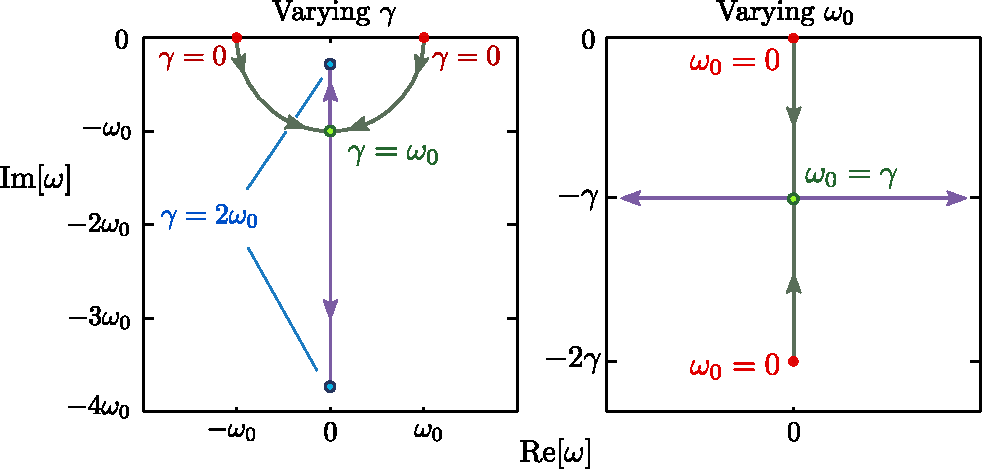
\includegraphics[width=0.76\textwidth]{oscillator_frequencies}
\end{figure}

Note the following features:

\begin{enumerate}
\item For $\gamma = 0$, the frequencies are both real, with values
  $\pm \omega_0$.

\item If we increase $\gamma$ from zero with $\omega_0$ fixed, both
  $\omega_+$ and $\omega_-$ move downwards in the complex plane, along
  a circular arc.

\item At $\gamma = \omega_0$, the frequencies meet along the imaginary
  axis.

\item For $\gamma > \omega_0$, the two frequencies move apart along
  the imaginary axis.
\end{enumerate}

To understand the implications of these complex frequencies, let
uswrite the real and imaginary parts of $\omega$ as $\omega_R + i
\omega_I$.  Then
\begin{align}
  z(t) = e^{-i\omega t} = e^{\omega_I t} \; e^{-i\omega_R t}.
\end{align}
If both $\omega_R$ and $\omega_I$ are non-zero, this describes a
spiral trajectory in the complex plane (see Section 3.6) whose
magnitude either increases or decreases with time, depending on the
sign of $\omega_I$.  To see this explicitly, we can write
\begin{align}
  z(t) = e^{\omega_I t} \, e^{-i\omega_R t}.
\end{align}
Taking the real part,
\begin{align}
  \mathrm{Re}\left[z(t)\right] = e^{\omega_I t} \, \cos\left[\omega_R t\right].
  \label{eq:Rez}
\end{align}

Assuming that $\gamma > 0$, the complex frequencies given by
Eq.~\eqref{eq:omegapm} always have $\omega_I < 0$.  Referring to
Eq.~\eqref{eq:Rez}, this means the solutions are always damped.
Moreover, if $\omega_R \ne 0$, then $z(t)$ executes a clockwise (for
$\omega_+$) or counterclockwise (for $\omega_-$) inward spiral; in
either case, $\mathrm{Re}[z(t)]$ describes an oscillation with
diminishing amplitude, consistent with our guess from
Section~\ref{damped-oscillations}.  On the other hand, if $\omega_R =
0$, then the solution is a pure exponential decay with no oscillation.
In the next few sections, we will undertake a systematic examination
of these two distinct behaviors.

\subsection{General solution for the damped harmonic oscillator}
\label{general-solution}

For now, let us suppose that $\omega_0 \ne \gamma$. Then we have two
distinct specific solutions,
\begin{align}
  z_\pm(t) = e^{-i\omega_\pm t}, \;\;\mathrm{where}\;\;\; \omega_\pm = -i\gamma \pm \sqrt{\omega_0^2 - \gamma^2}.
\end{align}
By taking a linear superposition of these specific solutions, we
obtain the general solution for the complex damped harmonic oscillator
equation:
\begin{align}
  z(t) = a_+ e^{-i\omega_+ t} + a_- e^{-i\omega_- t},
  \label{eq:gsol}
\end{align}
where $a_+$ and $a_-$ are independent complex free parameters.

(Note that if $\omega_0 = \gamma$, then $z_+(t) = z_-(t)$, so $a_+$
and $a_-$ would be coefficients multiplying the same function, and we
would not be allowed to treat them as two independent free
parameters. We will discuss how to handle this case in
Section~\ref{critical-damping}.)

To find solutions to the real damped harmonic oscillator equation, we
take $x(t) = \mathrm{Re}[z(t)]$. The resulting expression will depend
on whether $\omega_0 > \gamma$ or $\omega_0 < \gamma$. These two cases
lead to \textbf{under-damped solutions} and \textbf{over-damped
  solutions}, respectively, as discussed in the next two sections.

\subsubsection{Under-damped motion}
\label{underdamped}

First, consider $\omega_0 > \gamma$.  Let us define
\begin{align}
  \Omega = \sqrt{\omega_0^2 - \gamma^2} \in \mathbb{R},
\end{align}
so that $\omega_\pm = -i\gamma \pm \Omega$. Plugging this into the
complex general solution gives
\begin{align}
  z(t) &= a_+ e^{-\gamma t} e^{-i\Omega t} + a_- e^{-\gamma t} e^{i\Omega t} \\
  &= e^{-\gamma t} \left[a_+ e^{-i\Omega t} + a_- e^{i\Omega t} \right].
\end{align}
We can use Euler's formula to simplify the terms in the brackets:
\begin{align}
  a_+ e^{-i\Omega t} + a_- e^{i\Omega t} &= a_+ \big[\cos(\Omega t)-i\sin(\Omega t)\big] + a_- \big[\cos(\Omega t)+i\sin(\Omega t)\big] \\
  &= \big(a_+ + a_-\big) \cos(\Omega t) \;-\; i \big(a_+ - a_-\big) \sin(\Omega t).
\end{align}
Hence,
\begin{align}
  x(t) &= \mathrm{Re}\left[z(t)\right] \\
  &= e^{-\gamma t} \big[ A\cos\left(\Omega t\right) + B \sin\left(\Omega t\right) \big], \;\;\; \mathrm{where}\;\; \left\{\begin{aligned} A &= \mathrm{Re}\left[a_+ + a_-\right] \\
  B &= \mathrm{Im}\left[a_+ - a_-\right].\end{aligned}\right.
\end{align}
This is called an \textbf{under-damped solution}.  The coefficients
$A$ and $B$ are two independent \textit{real} parameters, so this
serves as a general solution for the real damped harmonic oscillator
equation. Using the trigonometric formulas, the solution can be
equivalently written as
\begin{align}
  x(t) = C \,e^{-\gamma t} \, \cos\!\big(\Omega t + \Phi\big), \;\;\;\mathrm{where}\;\;\left\{\begin{aligned}C &= \sqrt{A^2 + B^2}, \\ \Phi &= - \tan^{-1}\left[B/A\right].\end{aligned}\right.
\end{align}
This shows explicitly that it consists of a sinusoidal oscillation
(with frequency $\Omega$) overlaid on an ``envelope'' given by the
exponentially decreasing function $\exp(-\gamma t)$.  The graph of
$x(t)$ versus $t$ is plotted below:

\begin{figure}[ht]
  \centering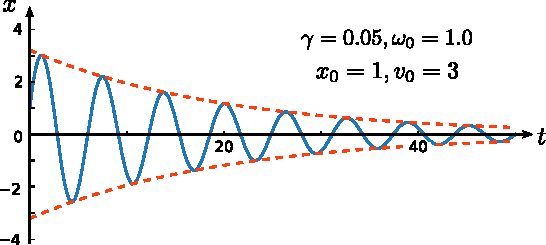
\includegraphics[width=0.61\textwidth]{underdamped}
\end{figure}

\subsubsection{Over-damped motion}
\label{overdamped}

For $\omega_0 < \gamma$, the square root term in $\omega_\pm =
-i\gamma \pm \sqrt{\omega_0^2 - \gamma^2}$ is imaginary.  Let us
define
\begin{align}
  \Gamma = \sqrt{\gamma^2 - \omega_0^2} \quad \Rightarrow \quad \omega_\pm = i \left(-\gamma \pm \Gamma\right).
\end{align}
Then the complex general solution can be simplified to
\begin{align}
  z(t) = a_+ e^{-\left(\gamma - \Gamma\right)\, t} + a_- e^{-\left(\gamma + \Gamma\right)\, t},
\end{align}
and the real solution is
\begin{align}
  x(t) &= \mathrm{Re}\left[z(t)\right] \\
  &= C_+ e^{-(\gamma - \Gamma) \,t} + C_- e^{-(\gamma + \Gamma) \, t},\;\;\;\mathrm{where}\;\; C_\pm = \mathrm{Re}[a_\pm].
\end{align}
This is called an \textbf{over-damped solution}.  It consists of two
exponentially decaying terms, with decay rates $(\gamma-\Gamma)$ and
$(\gamma + \Gamma)$ respectively. Since $\Gamma < \gamma$, both decay
rates are positive real numbers, but note that $(\gamma - \Gamma)$
\textit{decreases} with $\gamma$, whereas $(\gamma + \Gamma)$
\textit{increases} with $\gamma$, as shown below:

\begin{figure}[ht]
  \centering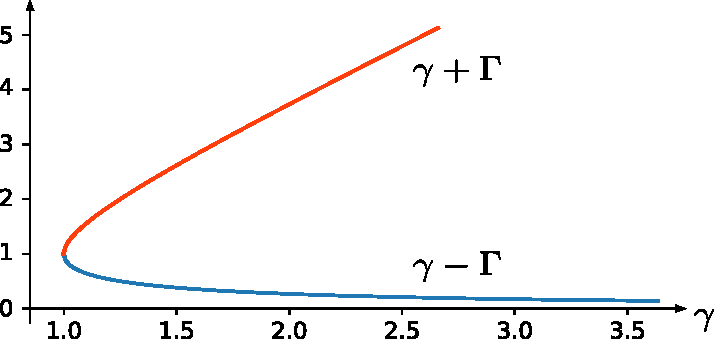
\includegraphics[width=0.5\textwidth]{decay_rates}
\end{figure}

Since $\gamma + \Gamma$ is associated with a faster-decaying
exponential, for large $t$ the second term becomes negligible compared
to the first term, and the solution has the limiting form
\begin{align}
  x(t) \approx C_+ e^{-(\gamma - \Gamma) t} \qquad (\mathrm{for}~\mathrm{large}~t).
\end{align}
A plot of $x(t)$ versus $t$ is shown below, with the limiting form
plotted as dashes.

\begin{figure}[ht]
  \centering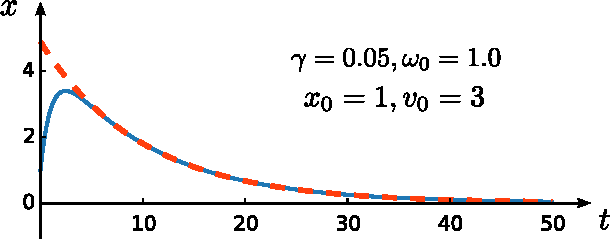
\includegraphics[width=0.55\textwidth]{overdamped}
\end{figure}

The over-damped solution has an interesting feature: \textit{for
  stronger damping, the decay rate at long times is slower}. This is
the opposite of the under-damped oscillator's behavior!
Mathematically, it happens because the decay rate $(\gamma-\Gamma)$,
appearing in the limiting form of $x(t)$ for large $t$, is a
decreasing function of $\gamma$.

In the over-damped regime, the motion of the oscillator is dominated
by the damping force rather than the spring force. Therefore, as the
oscillator tries to return to its equilibrium position $x = 0$, the
damping acts against this motion, and the stronger the damping, the
slower the decay to equilibrium. By contrast, in the under-damped
regime, the spring force is dominant, so stronger damping leads to
faster decay via faster dissipation of the oscillator's kinetic
energy.

\subsubsection{Critical damping}
\label{critical-damping}

\textbf{Critical damping} occurs when $\omega_0 = \gamma$.  Under this
special condition, the solution given in Eq.~\eqref{eq:gsol} reduces
to
\begin{align}
  z(t) = \left(a_+ + a_-\right) e^{-\gamma t}.
\end{align}
This has only \textit{one} independent complex parameter, i.e. the
parameter $(a_+ + a_-)$.  Therefore, it cannot be a general solution
for the complex damped harmonic oscillator equation.

We will not go into detail here regarding the procedure for finding
the general solution for the critically-damped oscillator, leaving it
as an exercise for the interested reader. Basically, it involves
Taylor expanding the solution near the critical point, and then
showing that there is a solution of the form
\begin{align}
  z(t) = \left(A + B t\right)\, e^{-\gamma t},
  \label{critical-sol}
\end{align}
which contains the desired two independent parameters.

The critically-damped solution contains an exponential decay constant
of $\gamma$, which is the same as the decay constant for the envelope
function in the under-damped regime (Section~\ref{underdamped}), and
\textit{larger} than the (long-time) decay constants in the
over-damped regime (Section~\ref{overdamped}).  Hence, we can regard
the critically-damped solution as the \textit{fastest-decaying
  non-oscillatory solution}.

This feature of critical damping is employed in many engineering
contexts, the most familiar being automatic door closers. If the
damping is too weak or the spring force is too strong (under-damped),
the door slams shut, whereas if the damping is too strong or the
spring force is too weak (under-damping), the door takes unnecessarily
long to swing shut. For best performance, an automatic door closer
should be tuned to a ``sweet spot'' that corresponds to the critical
point of a damped harmonic oscillator.

\subsection{Stating the solution in terms of initial conditions}
\label{stating-the-solution-in-terms-of-initial-conditions}

The general solution for the complex damped harmonic oscillator
equation contains two undetermined parameters which are the complex
amplitudes of the ``clockwise'' and ``counterclockwise'' complex
oscillations:
\begin{align}
  z(t) = a_+ e^{-i\omega_+ t} + a_- e^{-i\omega_- t}, \quad\mathrm{where} \;\; \omega_\pm =  -i\gamma  \pm \sqrt{\omega_0^2 - \gamma^2}.
\end{align}
However, mechanics problems are often expressed in terms of an
\textbf{initial value problem}, specifying the state of the system at
some initial time $t = 0$. In other words, given $z(0) \equiv x_0$ and
$\dot{z}(0) \equiv v_0$, what is $z(t)$ in terms of $x_0$ and $v_0$?

We can solve the initial-value problem by finding $z(0)$ and
$\dot{z}(0)$ in terms of the above general solution for $z(t)$:
\begin{align}
  z(0) &= \quad a_+ + a_- \qquad\quad= x_0 \\
  \dot{z}(0) &= -i\omega_+ a_+ - i \omega_- a_- = v_0.
\end{align}
These two equations can be combined into a $2\times2$ matrix equation:
\begin{align}
  \begin{bmatrix}1 & 1 \\ -i\omega_+ & -i\omega_-\end{bmatrix} \begin{bmatrix}a_+ \\ a_-\end{bmatrix} = \begin{bmatrix}x_0 \\ v_0\end{bmatrix}.
\end{align}
So long as $\omega_+ \ne \omega_-$, the matrix is non-singular, and we
can invert it to obtain $a_\pm$:
\begin{align}
  \begin{bmatrix}a_+ \\ a_-\end{bmatrix} = \frac{1}{i(\omega_+-\omega_-)}\begin{bmatrix}-i\omega_-x_0 - v_0 \\ i\omega_+x_0 + v_0 \end{bmatrix}.
\end{align}
We can plug these coefficients back into the general solution. After
some algebra, the result simplifies to
\begin{align}
  z(t) = e^{-\gamma t} \left[x_0 \cos(\Omega t) + \frac{\gamma x_0 + v_0}{\Omega} \, \sin(\Omega t)\right], \;\; \mathrm{where}\;\; \Omega \equiv \sqrt{\omega_0^2 - \gamma^2}.
\end{align}
For the under-damped case, $\Omega$ is real, and this solution is
consistent with the one we derived om Section~\ref{underdamped},
except that it is now explicitly expressed in terms our initial
conditions $x_0$ and $v_0$. As for the over-damped case, we can
perform the replacement
\begin{align}
  \Omega \rightarrow i \Gamma = i \sqrt{\gamma^2 - \omega_0^2}.
\end{align}

Then, using the relationships between trigonometric and hyperbolic
functions from Section 3.5.3, the solution can be re-written as
\begin{align}
  z(t) &= e^{-\gamma t} \left[x_0 \cosh(\Gamma t) + \frac{\gamma x_0 + v_0}{i\Gamma} \, i \sinh(\Gamma t)\right] \\
  &= \left(\frac{x_0}{2} + \frac{\gamma x_0 + v_0}{2\Gamma}\right) e^{-(\gamma - \Gamma) t} + \left(\frac{x_0}{2} - \frac{\gamma x_0 + v_0}{2\Gamma}\right) e^{-(\gamma+\Gamma)t},
\end{align}
which is consistent with the result found in Section~\ref{overdamped}.

In either case, so long as we plug in real values for $x_0$ and $v_0$,
the solution is guaranteed to be real for all $t$.  That's to be
expected, since the real solution is also one of the specific
solutions for the complex harmonic oscillator equation.

\subsection{Exercises}
\label{exercises}

\begin{enumerate}
\item
  In Section~\ref{complex-frequencies}, we encountered the complex
  frequencies
  \begin{equation}
    \omega_\pm = -i\gamma \pm \sqrt{\omega_0^2 - \gamma^2}.
  \end{equation}
  For fixed $\omega_0$ and $\omega_0 > \gamma$ (under-damping), prove
  that $\omega_\pm$ lie along a circular arc in the complex plane.

\item
  Derive the general solution for the critically damped harmonic
  oscillator by following these steps:
  \begin{enumerate}[(a)]
  \item
    Consider the complex ODE, in the under-damped regime $\omega_0 >
    \gamma$. We saw in Section~\ref{general-solution} that the general
    solution has the form
    \begin{equation}
      z(t) = \psi_+ \, \exp\left[\left(-\gamma  - i \sqrt{\omega_0^2 - \gamma^2}\right)t\right] \; +\; \psi_- \, \exp\left[\left(-\gamma +i\sqrt{\omega_0^2 - \gamma^2}\right)t\right]
    \end{equation}
    for some complex parameters $\psi_+$ and $\psi_-$. Define the
    positive parameter $\varepsilon = \sqrt{\omega_0^2 - \gamma^2}$.
    Re-write $z(t)$ in terms of $\gamma$ and $\varepsilon$ (i.e.,
    eliminating $\omega_0$).

  \item
    The expression for $z(t)$ is presently parameterized by the
    independent parameters $\psi_+$, $\psi_-$, $\varepsilon$, and
    $\gamma$. We are free to re-define the parameters, by taking
    \begin{align}
      \alpha &= \psi_+ + \psi_- \\
      \beta &= -i\varepsilon(\psi_+ - \psi_-).
    \end{align}
    Using these equations, express $z(t)$ using a new set of
    independent complex parameters, one of which is $\varepsilon$.
    Explicitly identify the other independent parameters, and state
    whether they are real or complex.
  \item
    Expand the exponentials in $z(t)$ in terms of the parameter
    $\varepsilon$. Then show that in the limit $\varepsilon
    \rightarrow 0$, $z(t)$ reduces to the critically-damped general
    solution \eqref{critical-sol}.
  \end{enumerate}

\item
  Repeat the above derivation for the critically-damped solution, but
  starting from the over-damped regime $\gamma > \omega_0$.

\item
  Let $z(t)$ be a complex function of a real input $t$, which obeys
  the differential equation
  \begin{equation}
    \frac{dz}{dt} = -i\,(\omega_1 - i \gamma)\; z(t),
  \end{equation}
  where $\omega_1$ and $\gamma$ are real. Find the general solution
  for $z(t)$, and hence show that $z(t)$ satisfies the damped
  oscillator equation
  \begin{equation}
    \left[\frac{d^2}{dt^2} + 2\gamma \frac{d}{dt} + \omega_0^2 \right] z(t) = 0
  \end{equation}
  for some $\omega_0^2$. Finally, show that this harmonic oscillator
  is always under-damped.
  \vskip -0.05in
  \hfill{\scriptsize [solution~available]}
\end{enumerate}


\end{document}
